\documentclass{ctexart}
\CTEXsetup[format={\Large\bfseries}]{section}
\newcommand{\jn}{JN}
\usepackage{graphicx}
\usepackage{float}

\begin{document}

\title{学习笔记--istio}
\author{mayidudu 来自 \jn}
\maketitle
%https://blog.csdn.net/wcx1293296315/article/details/79775671, 插图



\section{istio是什么}
一个用来连接、管理和保护微服务的开放平台。 
Istio提供一种简单的方式来建立已部署服务网络,具备负载均衡、服务间认证、监控等功能,而不需要改动任何服务代码。 
想要为服务增加对Istio的支持,您只需要在环境中部署一个sidecar,使用Istio控制面板功能配置和管理代理,拦截微服务之间的所有网络通信。
\section{istio与spring cloud比较}
istio是无侵入式的,可以支持多语言,而spring cloud是针对java平台的。

\section{istio的架构}
\begin{figure}[H]
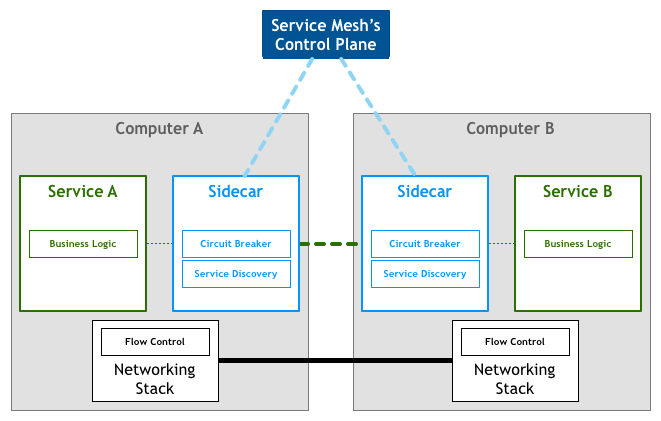
\includegraphics[scale=0.6]{istio/framework.png}
\caption{istio架构}
\end{figure}

\section{Istio的主要功能}
流量管理(Pilot)。控制服务之间的流量和API调用的流向,使得调用更灵活可靠,并使网络在恶劣情况下更加健壮。

可观察性。通过集成zipkin等服务,快速了解服务之间的依赖关系,以及它们之间流量的本质和流向,从而提供快速识别问题的能力。

策略执行(mixer)。将组织策略应用于服务之间的互动,确保访问策略得以执行,资源在消费者之间良好分配。策略的更改是通过配置网格而不是修改应用程序代码。

服务身份和安全(Istio-auth)。为网格中的服务提供可验证身份,并提供保护服务流量的能力,使其可以在不同可信度的网络上流转。

除此之外,Istio针对可扩展性进行了设计,以满足不同的部署需要:

平台支持。Istio旨在可以在各种环境中运行,包括跨云、预置环境、Kubernetes、Mesos等。最初专注于Kubernetes,但很快将支持其他环境。
集成和定制。策略执行组件可以扩展和定制,以便与现有的ACL、日志、监控、配额、审核等解决方案集成。

\section{istio分层}
分为控制平面和数据平面两部分。 
\begin{enumerate}
	\item [-] 控制平面:Pilot, Mixer, Istio-Auth,分别对Istio中的服务做流量管理,策略配置,安全通信等规则配置 
	\item [-] 数据平面:所有pod上的Envoy,负责所有规则的执行
\end{enumerate}
\begin{figure}[H]
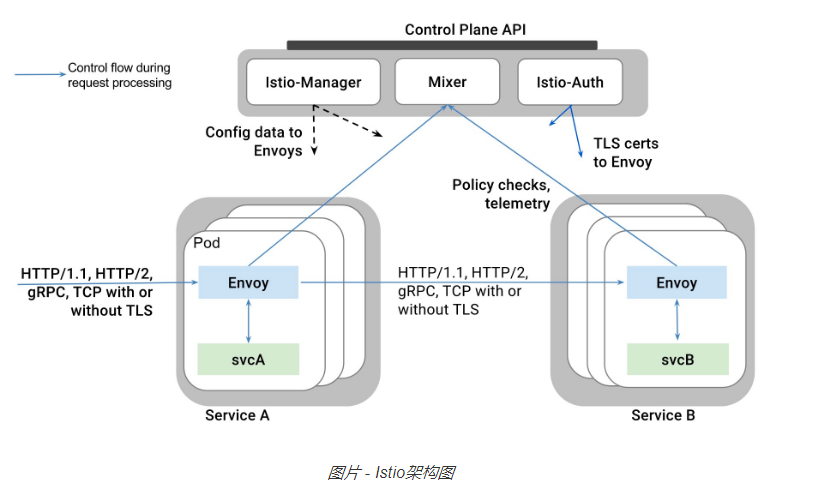
\includegraphics[scale=0.5]{istio/framework2.png}
\caption{istio分层结构}
\end{figure}

\section{Istio 服务无法访问外网问题}
缺省情况下,启用了Istio的服务是无法访问外部URL的,这是因为Pod中的iptables把所有外发传输都转向到了Sidecar代理,而这一代理只处理集群内的访问目标。

我们可在Istio集群中使用两种方式来访问外部服务:
使用Egress规则。
配置Istio Sidecar,在他的iptables中排除对外部IP的控制。 
Egress 规则
配置Istio Sidecar 
让指定IP范围直接穿透Istio,就需对源服务的Envoy Sidecar进行配置,阻止其对外部请求的拦截。

通过--includeIPRanges指定。

% kubectl apply -f <(istioctl kube-inject -f samples/sleep/sleep.yaml --includeIPRanges=10.0.0.1/24)

%IPranges即service的IP范围,在kube-api_server.service中通过–service-cluster-ip-range指定。

\end{document}